% Method section for the BISON manuscript.
% Author: fangtoast
% Email: fangtoast@foxmail.com
% Copyright (c) 2026 fangtoast. All rights reserved.

\section{Method}

\subsection{Band-Informed Spectral Operator}

BISON consumes \(\permittivity\) as a one-channel periodic field. A
\(1\times1\) convolution first lifts it to \(C\) latent channels,
\(\mathbf{u}_0=P\permittivity\). Four BandBlocks then update the field. In
block \(\ell\), the spectral path is
\begin{equation}
  \mathbf{s}_{\ell}=\mathcal{F}^{-1}\!\left[
  \left(R^{\mathrm{full}}_{\ell}+R^{\mathrm{band}}_{\ell}\right)
  \mathcal{F}(\mathbf{u}_{\ell})\right],
  \label{eq:dual-spectral}
\end{equation}
where both complex kernels act on configured low-frequency rectangles, with
the band kernel using a separately configured subset. The two kernels are
learned independently and added in Fourier space. A pointwise convolution is
combined with this global path, then modulated by a learned sigmoid gate:
\begin{align}
  \mathbf{a}_{\ell}&=\mathbf{s}_{\ell}+W_{\ell}\mathbf{u}_{\ell},\\
  \widetilde{\mathbf{a}}_{\ell}
  &=\sigma(G_{\ell}\mathbf{a}_{\ell})\odot\mathbf{a}_{\ell}.
\end{align}
A low-rank global branch pools the residual field, applies
\(C\rightarrow r\rightarrow C\) channel maps, and broadcasts the result.
The block output is
\begin{equation}
  \mathbf{u}_{\ell+1}=\operatorname{GELU}\!\left(
  S_{\ell}[\widetilde{\mathbf{a}}_{\ell}+L_{\ell}(\mathbf{u}_{\ell})]
  +\mathbf{u}_{\ell}\right).
  \label{eq:bandblock}
\end{equation}
Adaptive global pooling followed by a linear head reshapes the final channels
to \(\bandpred\in\mathbb{R}^{N_k\times N_b}\). In the evaluated configuration,
\(C=32\), \(r=8\), the two spectral rectangles retain \(8\times8\) and
\(5\times5\) modes, four BandBlocks are stacked, and the network contains
389,718 trainable parameters. Both Fourier weights are complex-valued and are
cropped at runtime when the data grid provides fewer available modes.

Figure~\ref{fig:bison-detailed} expands this implemented operator at both the
network and block levels. It makes explicit that the band gate acts on the
sum of the global spectral and local pointwise paths, while the pooled
low-rank branch is computed from the block input and broadcast before the
learned projection and identity residual.

\begin{figure*}[t]
  \centering
  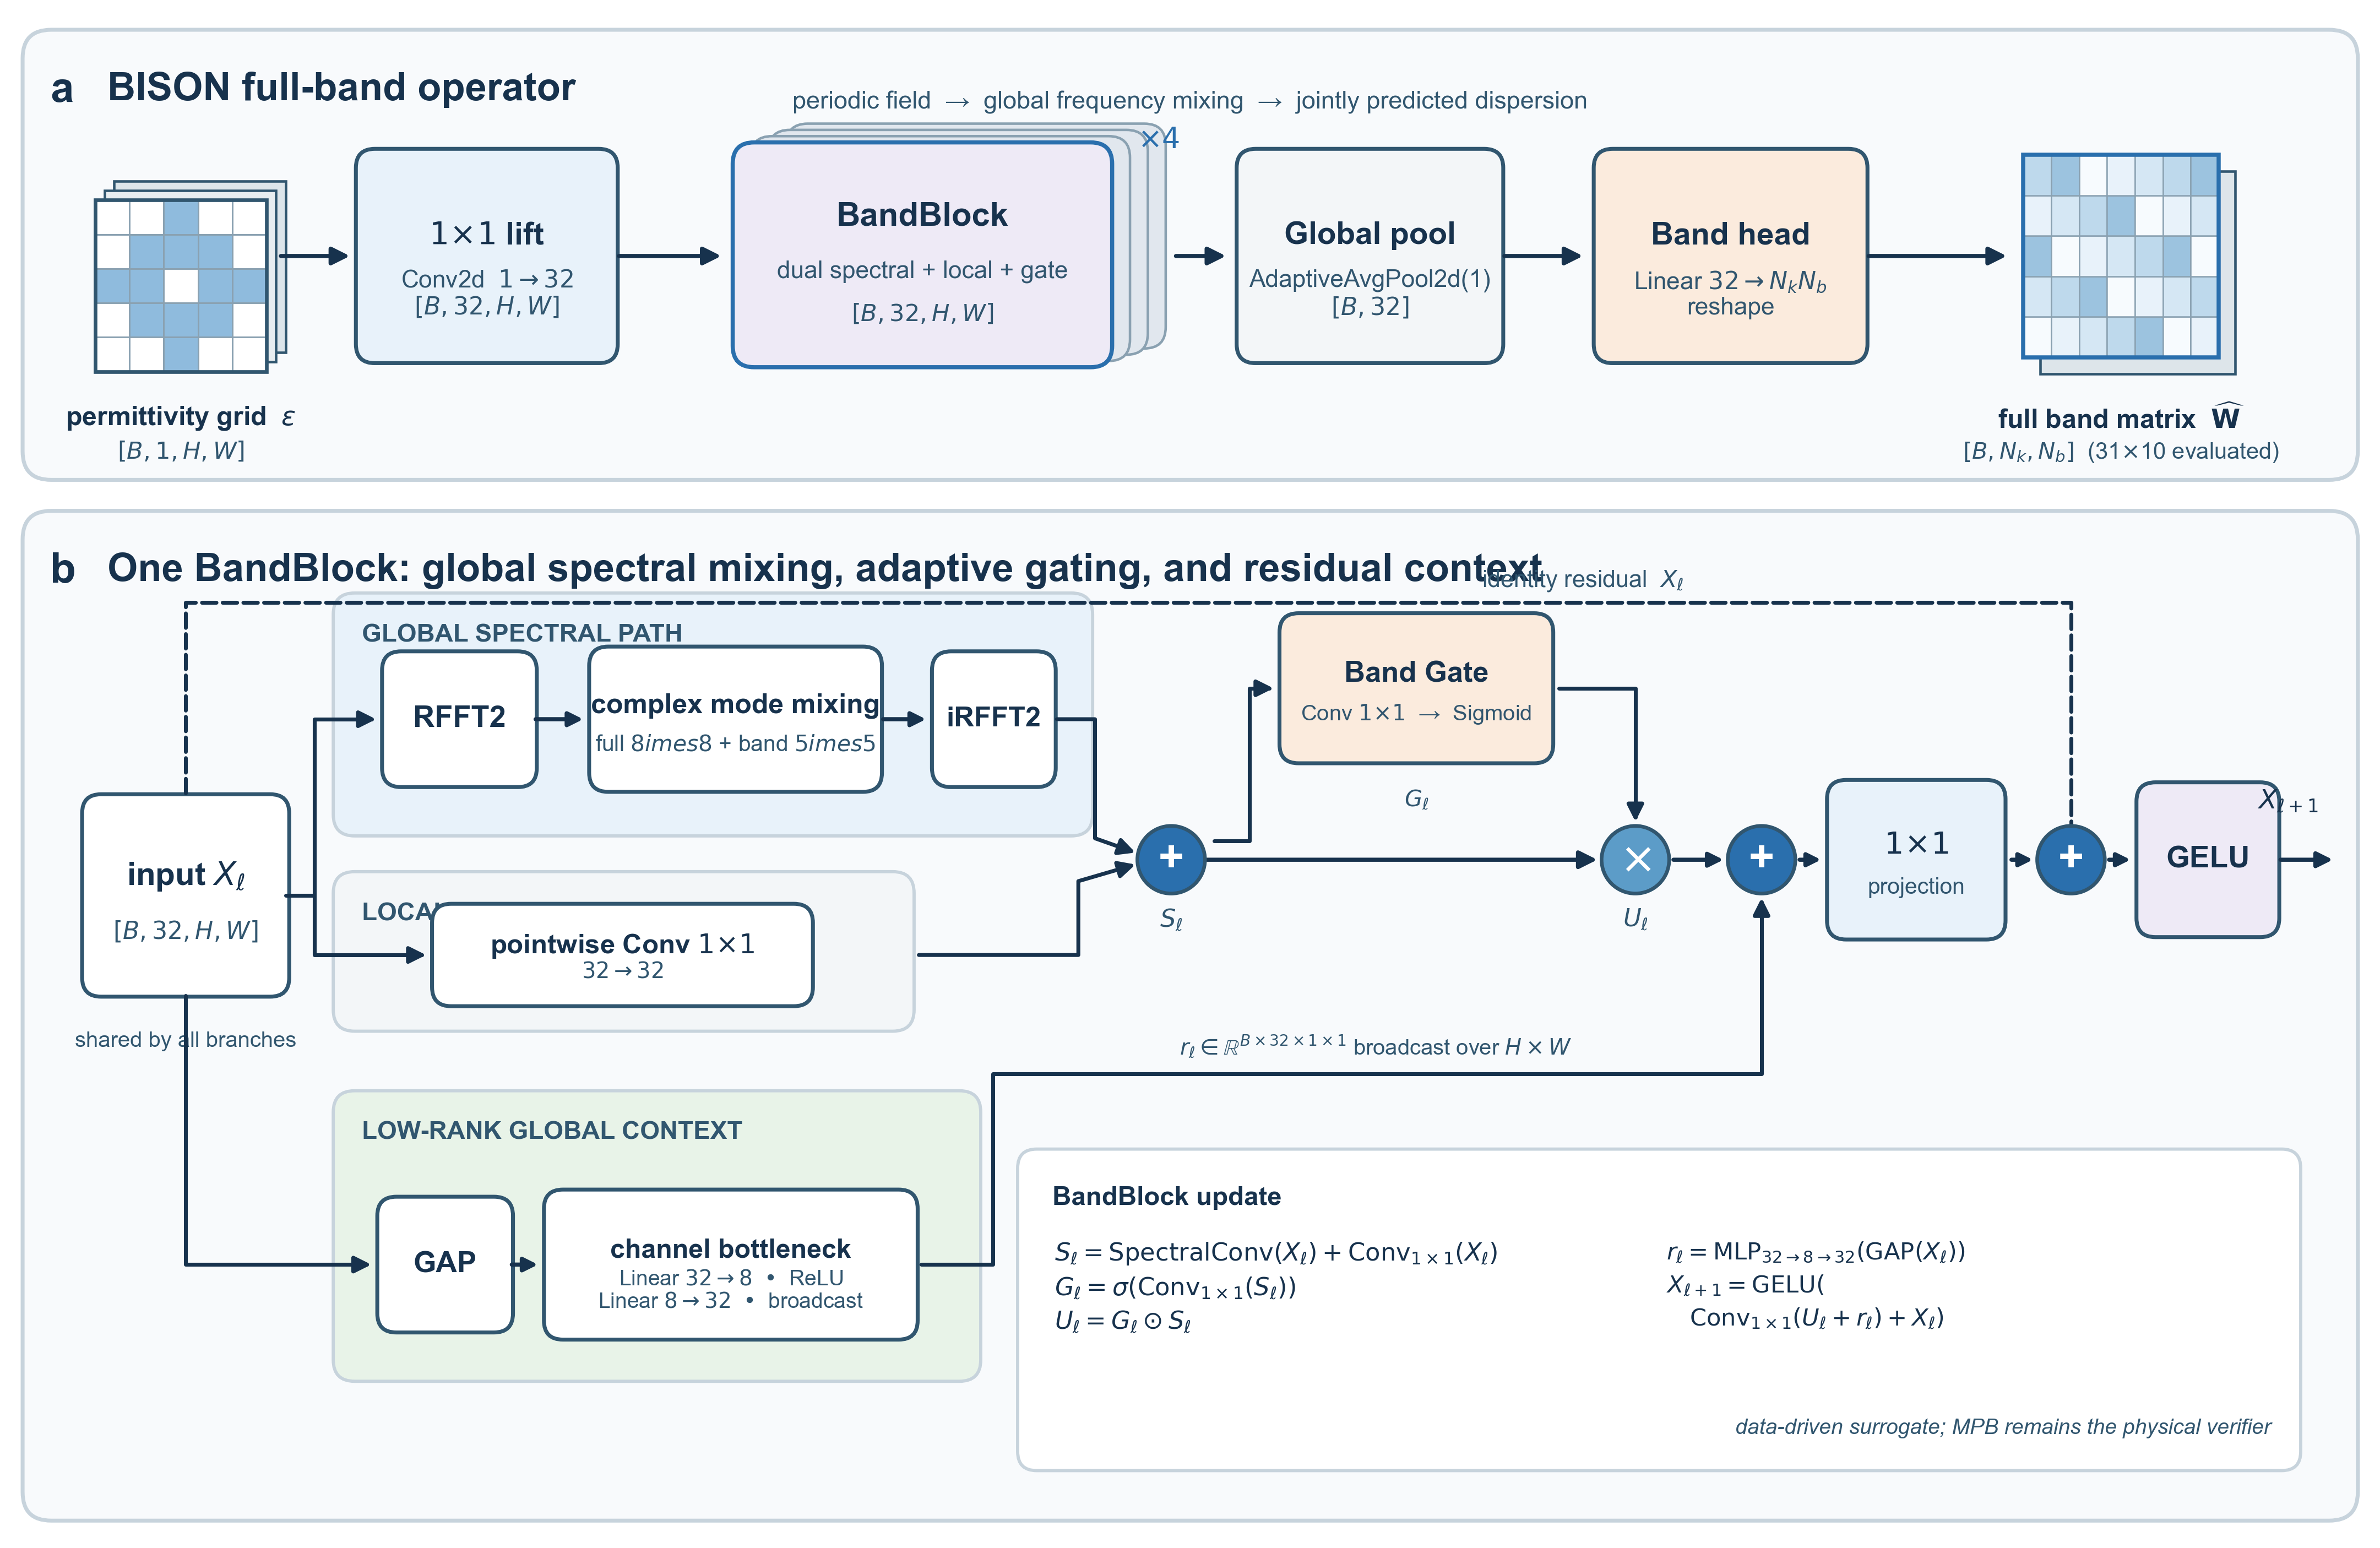
\includegraphics[width=\textwidth]{figures/bison_architecture_detailed.png}
  \caption{Detailed architecture of the BISON forward operator.
  \textbf{(a)} A periodic permittivity grid is lifted to \(C=32\) channels,
  processed by four BandBlocks, globally pooled, and mapped jointly to the
  ordered \(N_k\times N_b\) band matrix (\(31\times10\) in the evaluated A1
  data). \textbf{(b)} Inside one BandBlock, an RFFT2 branch mixes two learned
  complex low-mode rectangles (configured as \(8\times8\) and \(5\times5\))
  and is added to a local \(1\times1\) path. A sigmoid channel gate modulates
  this mixed field. In parallel, global average pooling and the
  \(32\rightarrow8\rightarrow32\) bottleneck produce a broadcast context
  vector. Their sum passes through a learned \(1\times1\) projection before
  the identity residual and GELU activation. The diagram follows the actual
  implementation order; it depicts a data-driven surrogate rather than an
  embedded MPB or Maxwell solver.}
  \Description{A two-panel architecture diagram. Panel a shows a permittivity
  grid flowing through a one-by-one lift, four stacked BandBlocks, global
  pooling, and a linear band head to a full band matrix. Panel b expands a
  BandBlock into spectral, pointwise, gating, low-rank global-context,
  projection, residual, and activation paths.}
  \label{fig:bison-detailed}
\end{figure*}

The architecture is FNO-derived rather than a separate physics solver. Its
inductive bias is that periodic geometry and long-range interactions are
processed globally in Fourier space, while the full ordered band matrix is
predicted jointly. This paper uses the name BISON for this exact implemented
model, not for a hypothetical replacement architecture.

The term \emph{band-informed} refers to this task specialization, not to a
hard-coded Maxwell constraint. The second spectral kernel gives the block a
separate learnable low-mode scale; the sigmoid gate determines which mixed
channels are passed onward; and the pooled bottleneck injects a cell-wide
summary before the residual update. Their combined output is learned solely
from paired permittivity--band data. Consequently, the architecture can be a
fast spectral surrogate, but its predictions still require calibration and
solver replay when used outside ordinary held-out forward evaluation.

\subsection{Independent Query-Operator Audit}

The project also trains \(\queryop(\permittivity,\mathbf{k})\), which returns
the band vector at a physical Bloch coordinate. It is evaluated on all sampled
queries, interpolation points withheld from otherwise observed path segments,
and a completely held-out path segment. During inverse evaluation, BISON is
the primary objective and ranker; \(\queryop\) is a diagnostic consistency
gate. This asymmetric use avoids presenting agreement between two learned
models as physical verification.

\subsection{Single-Mode No-Expert Candidate Generator}

For inverse design, the target matrix is flattened and encoded by two
GELU-activated linear layers. The encoded condition is concatenated with a
32-dimensional Gaussian latent vector and one fixed mode embedding, then
decoded by a four-layer, width-256 MLP with a sigmoid output. Setting the mode
count to one removes routing and expert selection: every draw is processed by
the same parameters and differs only through its continuous latent vector.
The output represents the independent degrees of freedom of the symmetric
binary design; deterministic lifting and thresholding recover the complete
\(\pgroup\) unit cell.

The inverse model is warm-started from paired reconstruction and then optimized
for 50 epochs with AdamW while BISON and the query operator remain frozen. For
16 latent candidates per training condition, the objective is
\begin{equation}
\begin{split}
  \mathcal{L}={}&\mathcal{L}_{\mathrm{BISON}}
  +0.03\mathcal{L}_{\mathrm{rec}}
  +0.20\mathcal{L}_{\mathrm{div}}
  +0.50\mathcal{L}_{\mathrm{bin\text{-}div}}\\
  &+0.25\mathcal{L}_{\mathrm{latent}}
  +0.90\mathcal{L}_{\mathrm{collision}}
  +0.20\mathcal{L}_{\mathrm{cross}}
  +0.20\mathcal{L}_{\mathrm{gap}}.
  \label{eq:inverse-objective}
\end{split}
\end{equation}
The terms promote target fidelity, paired warm-start stability, continuous and
binary diversity, latent responsiveness, separation from near-duplicate
structures, and agreement between the two frozen surrogates. MPB gradients are
not used.

This generator is intentionally subordinate to BISON in the paper's method
identity. BISON defines the learned full-band objective; the generator proposes
points in the legal design space. Calling the combined system a mixture of
experts would be misleading because the selected method has one fixed mode,
one decoder, and no learned router. The four-mode version is retained only as a
same-implementation baseline for testing whether discrete mode embeddings add
value under an identical sampling budget.

\subsection{Candidate Ranking and Solver Replay}

At inference, each target receives \(K=128\) latent draws. Candidates are
thresholded at 0.5, checked for legality, and deduplicated using a normalized
Hamming threshold determined by the geometry degrees of freedom. Frozen BISON
ranks the surviving pool by bands-2--10 MRE; the query model records an
independent diagnostic score. The five best BISON-ranked candidates are then
recomputed by MPB, and the lowest real-MPB MRE is reported. The mode-count-four
generator is evaluated only as a same-budget baseline. It is not part of
BISON and is not required by the proposed no-expert workflow.
